\documentclass[a4paper,10pt,headings=normal,bibliography=totoc]{scrartcl}

\usepackage{scrhack}  % Fix a LaTeX warning

%%%%%%%%%%%%%%%%%%%%%%%%%%%%%%%%%%%%%%%%%%%%%%%%%%%%%%%%%%%%%%%%%%%%%%%%%%%%%%%
\usepackage[utf8x]{inputenc}
\usepackage{amsmath}
\usepackage{amssymb}
\usepackage{amsthm}
\usepackage{bm}
\usepackage{colonequals}
\usepackage{overpic}
\usepackage{url}
\usepackage{xspace}
\usepackage[square,numbers,sort]{natbib}

\usepackage[colorinlistoftodos]{todonotes}
%\usepackage[colorinlistoftodos,disable]{todonotes}
\usepackage{environ}
\usepackage{enumitem}
\usepackage{listings}
\usepackage{float}


\usepackage{tikz}
\usetikzlibrary{arrows}
\tikzset{
    treenode/.style = {
        align=center,
        inner sep=0pt,
        text centered,
        font=\sffamily,
        rectangle,
        rounded corners=3mm,
        draw=black,
        minimum width=2em,
        minimum height=2em
    },
    basisnode/.style = {
        treenode,
        rectangle,
        rounded corners=3mm,
    }
}


%%%%%%%%%%%%%%%%%%%%%%%%%%%%%%%%%%%%%%%%%%%%%%%%%%%%%%%%%%%%%%%%%%%%%%%%%%%%%%%
%%%%%%%%%%%   hyperref should be loaded late to avoid incompatibilities
\usepackage[pdftitle={Function space bases in the dune-functions module},
            pdfauthor={Christian Engwer, Carsten Gräser, Steffen Müthing, and Oliver Sander}]
             {hyperref}

\usepackage{attachfile2}
\usepackage{fancyvrb}

%%%%%%%%%%%%%%%%%%%%%%%%%%%%%%%%%%%%%%%%%%%%%%%%%%%%%%%%%%%%%%%%%%%%%%%%%%%%%%%
%%%%%%%%%%%%     Settings for the listings package
\lstset{language={c++},
         basicstyle=\ttfamily\small,
%         basicstyle=\small,
         commentstyle=\textit,
%         columns=fixed,
         columns=flexible,
         escapeinside={/*@}{@*/}
        }

% How to include ranges of an external source code file
\lstset{rangeprefix=//\ \{\ ,% curly left brace plus space, all in a C++-style comment
        rangesuffix=\ \},% space plus curly right brace
        numberstyle=\footnotesize,  % font size for numbers
        includerangemarker=false}  % Do not show the range markers

\newcommand{\cpp}[1]{\lstinline[basicstyle=\ttfamily]!#1!}


\newtheorem{definition}{Definition}

%%%%%%%%%%%%%%    Define a 'shellenv' environment for shell output
\usepackage{fancyvrb}

\DefineVerbatimEnvironment%
 {shellenv}{Verbatim}
 {}


%%%%%%%%%%%%%%%%%%%%%%%%%%%%%%%%%%%%%%%%%%%%%%%%%%%%%%%%%%%%%%%%%%%%%%%%%%%%%%%

\newcommand{\R}{\mathbb{R}}
\newcommand{\N}{\mathbb{N}}
\newcommand{\abs}[1]{{\lvert#1\rvert}}
\newcommand{\norm}[1]{\lVert#1\rVert}
\newcommand{\op}[1]{\operatorname{#1}}
\newcommand{\st}{\; : \;}
\renewcommand{\div}{\operatorname{div}}
\DeclareMathOperator{\trace}{tr}

\newcommand{\dune}{\textsc{Dune}\xspace}
\newcommand{\program}[1]{\textsc{#1}\xspace}



% For typesetting Dune module names
\newcommand{\dunemodule}[1]{\texttt{#1}}
% For typesetting file names
\newcommand{\file}[1]{\texttt{#1}}


%%  All graphics files must be in this subdirectory
\graphicspath{{gfx/}}

%%%%%%%%%%%%%%%%%%%%%%%%%%%%%%%%%%%%%%%%%%%%%%%%%%%%%%%%%%%%%%%%%%%%%%%%%%%%%%%%%%%%%%%%%%%%%%%%%%%%%
%%%%%%%%%%%%%%%%%%%%%%%%%%%%%%%%%%%%%%%%%%%%%%%%%%%%%%%%%%%%%%%%%%%%%%%%%%%%%%%%%%%%%%%%%%%%%%%%%%%%%
%%%%%%%%%%%%%%%%%%%%%%%%%%%%%%%%%%%%%%%%%%%%%%%%%%%%%%%%%%%%%%%%%%%%%%%%%%%%%%%%%%%%%%%%%%%%%%%%%%%%%

\title{Function space bases in the dune-functions module}
\author{Christian Engwer, Carsten Gräser, Steffen Müthing, and Oliver Sander}
%\date{}

\begin{document}

\maketitle

\tableofcontents

\begin{abstract}
 \dunemodule{dune-functions} is a \dune module that provides interfaces for functions and function space bases.
 It forms one abstraction level above grids, shape functions, and linear algebra, but still sits below
 full discretization frameworks like \dunemodule{dune-pdelab} and \dunemodule{dune-fem}.
 As an example, this document shows how the \dunemodule{dune-functions} module can be used to solve the Stokes
 equation with a Taylor--Hood discretization.
\end{abstract}

\section{Introduction}


The main purpose of the \dunemodule{dune-functions} module is to describe discrete function spaces defined on a grid.
Still, the central concept in the code is not the function space itself, but rather the {\em basis} of the function space.
This is because even though finite element spaces play a central role in theoretical considerations of the FE method,
actual computations are done using coefficients, given with respect to a particular basis.  Also,
for many different finite element spaces, more than one basis is used in practice.  For example,
the space of second-order Lagrangian finite elements is used both with the nodal (Lagrange) basis, and with the
hierarchical basis~\cite{bank:1996}.  Discontinuous Galerkin spaces can be described in terms of Lagrange bases,
monomial bases, Legendre bases and more.  It is therefore important to be able to distinguish these different
representations of the same space in the application code.

Finite element function space bases frequently exhibit a fair amount of structure.  Vector-valued spaces can be
written as products of scalar spaces, and the same holds for mixed finite elements.  Even more, such spaces
have a natural structure as a tree, with scalar-valued or otherwise irreducible spaces forming the leaves, and
products forming the other nodes.

This abstract construction is described in Chapter~\ref{sec:dune_functions:finite_element_trees}.
The programmer interface is centered around this notion of trees of finite element spaces, and gains
much elegance from it.
Then, Chapter~\ref{sec:dune_functions:function_space_bases_implementation} explains the programmer interface to function space bases.

The \dunemodule{dune-functions} module also contains an the interface for functions.
This interface is described in a separate paper~\cite{engwer_graeser_muething_sander:2015}.

\subsection{Obtaining and installing the module}

The code for the \dune interface for function spaces and functions
described in this chapter is contained in a separate \dune module called \dunemodule{dune-functions}.
Consequently, all header include paths
start with \cpp{dune/functions/}, and all code is contained in the namespace \cpp{Dune::Functions}.
In addition, \dunemodule{dune-functions} depends on a library for tree data structures contained in a module
called \dunemodule{dune-typetree}, which needs to be available to use \dunemodule{dune-functions}.
If you have not installed the two modules already, please do so now.  On Linux systems you may get them
from your distribution.  Otherwise, download the source code by
\begin{shellenv}
git clone http://git.dune-project.org/repositories/dune-typetree
git clone http://git.dune-project.org/repositories/dune-functions
\end{shellenv}
Then you can build both modules in the usual way, by calling
\begin{shellenv}
dunecontrol all
\end{shellenv}



\section{Function space bases}
\label{sec:dune_functions:finite_element_trees}


Before we can explain the implementation of bases for discrete function spaces in Chapter~\ref{sec:dune_functions:function_space_bases_implementation},
we need to say a few words about the general structure of such spaces.  Given one or several finite element bases
with basis functions taking values in different Euclidean spaces,
\dunemodule{dune-functions} allows to systematically construct bases for function spaces with a
higher-dimensional range.  These include vector-valued functions, mixed finite elements, and spaces
for multi-physics.  The building blocks are typically scalar-valued basis functions, but sometimes vector-valued
ones like the N\'ed\'elec basis are used as well. The constructions are systematically described as tree structures.
This tree construction of finite element spaces has first been systematically worked out in~\cite{muething:2015}.

Readers who are only interested in scalar finite element spaces may try to proceed directly to
Chapter~\ref{sec:dune_functions:function_space_bases_implementation}.  They should only know that whenever a tree
is mentioned there, this tree consists of a single node only, which is the FE basis.

\subsection{Trees of finite element spaces}

Throughout this chapter we assume that we have a single fixed domain $\Omega$, and all function spaces
that we consider are defined on this domain.
There are primarily two ways how two bases can be combined to form a new one:
Internal sums and external sums.

Some finite element spaces arise naturally as the internal sum of two simpler ones.
I.\,e., both have the same range space $R$ and are thus subspaces of the space $R^\Omega$
of all functions mapping from $\Omega$ to $R$. Then the internal sum is just the classic
sum in $R^\Omega$.  The sum space will have that same range space.
If the sum is direct, then a basis of the sum is given by the union of the bases of
the simpler ones.
For example,
a $P_2$-space can be viewed as a $P_1$-space plus a hierarchical extension consisting of bubble functions.
XFEM spaces~\cite{moes_dolbow_belytschko:1999} are constructed by adding special basis functions to a basic space to capture
free discontinuities.
If an internal sum is direct, then it can, up to an isomorphism, also be written as
an external sum as described below.
%The two spaces in such a sum must have the same range space.
The \dunemodule{dune-functions} module does not currently support marking the sum
of finite element bases to be internal.

The second way to construct FE spaces from simpler ones is by building external sums or,
equivalently, Cartesian products of FE spaces.  This is what
\dunemodule{dune-functions} focuses on, and we will describe it in a bit more detail.
Let $B = \{b_i\}_{i=1}^{n_1}$ and $C = \{c_i\}_{i=1}^{n_2}$ be two scalar function space bases and let $\mathbf{e}_1$, $\mathbf{e}_2$ be the canonical
basis vectors in $\R^2$.
Then we define the external sum or Cartesian product of the spanned spaces $\op{span}B$ and $\op{span} C$ as
\begin{align*}
    \operatorname{span} B \oplus \operatorname{span} C
    = \operatorname{span} B \times \operatorname{span} C
    = \big\{ (v,w) \st v \in \op{span} B, w \in \op{span} C \big\}.
\end{align*}
A natural basis of this space is given by the concatenation
of the bases $B$ and $C$ defined by
\begin{align*}
(B,C)
 & \colonequals
    \mathbf{e}_1 \otimes B \cup \mathbf{e}_2 \otimes C \\
    &= \big\{ \mathbf{e}_1 \otimes b \st b \in B \big\}
    \cup \big\{ \mathbf{e}_2 \otimes c \st c \in C \big\} \\
 & =
 \big\{(b_1,0), (b_2,0), \dots, (b_{n_1},0) \big\} \cup \big\{(0,c_1), (0,c_2), \dots, (0,c_{n_2})\big\}.
\end{align*}
These basis functions take values in $\R \times \R = \R^2$.
More generally, if $B$ and $C$ are bases with ranges $\R^{m_1}$
and $\R^{m_2}$, respectively, then
\begin{equation*}
    (B,C)
 \colonequals
 \big\{(b_1,\underbrace{0}_{\in \R^{m_2}}), (b_2,\underbrace{0}_{\in \R^{m_2}}), \dots, (b_{n_1},\underbrace{0}_{\in \R^{m_2}})\big\}
 \cup
 \big\{(\underbrace{0}_{\in \R^{m_1}}, c_1), (\underbrace{0}_{\in \R^{m_1}},c_2), \dots, (\underbrace{0}_{\in \R^{m_1}}, c_{n_2})\big\}
\end{equation*}
is again the natural basis of the space $\operatorname{span} B \oplus \operatorname{span} C$.  Its basis functions take values in
$\R^{m_1} \times \R^{m_2} = \R^{m_1+m_2}$.

It is important to note that building the external sum of vector spaces
corresponds to building the Cartesian product of the sets which should not
be confused with building the tensor product of these spaces.
It is however true, that the $k$-fold product or $k$-th power
of a single space can be viewed as the tensor product with $\R^k$, i.e,
\begin{align*}
    (\op{span} B)^k
    = \underbrace{\op{span}B \times \dots \times \op{span}B}_{k-\text{times}}
    = \underbrace{\op{span}B \oplus \dots \oplus \op{span}B}_{k-\text{times}}
    = \R^k \otimes \op{span} B.
\end{align*} 
In the following we will simply use the term \emph{product}
when we talk about the Cartesian product or external sum.

The construction via products (external sums) allows to build vector-valued and mixed finite element spaces of arbitrary complexity.
For example, the space of
first-order Lagrangian finite elements with values in $\R^3$ can be seen as the product $P_1 \times P_1 \times P_1$.
The simplest Taylor--Hood element is the product $(P_2)^3 \times P_1$
of $(P_2)^3 = P_2 \times P_2 \times P_2$ for the velocities with $P_1$ for the pressure.
If more physical quantities need to be dealt with, more factor bases can be included easily.  Note also that we have not
required that these spaces be defined with respect to the same grid (or any grid at all, for that matter).

For any spaces used in FE simulations that can be written as a product, there is an order of the factors that appears more natural
than others.  For example, the Taylor--Hood space is usually written as $P_2 \times P_2 \times P_2 \times P_1$,
even though $P_2 \times P_1 \times P_2 \times P_2$ would work as well.  The reason is that the triple
$P_2 \times P_2 \times P_2$ forms a semantic unit---it contains the components of a velocity field.
This, together with the associativity of the product of spaces, allows to even write this
as $(P_2 \times P_2 \times P_2) \times P_1$.  This grouping makes the semantic relationship even clearer.

Grouped expressions of this type are conveniently visualized as tree structures.  This
suggests to interpret composite
finite element spaces as tree structures.  In this structure, leaf nodes represent scalar or otherwise irreducible spaces,
and inner nodes represent products of their children.  Subtrees then represent composite
finite element spaces.  Figure~\ref{fig:dune_functions:taylor_hood_basis_tree} shows the Tayor--Hood finite element
space in such a tree representation.

\begin{figure}
    \begin{center}
        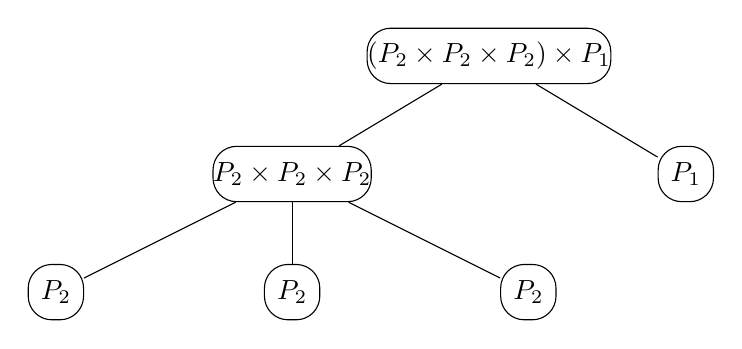
\begin{tikzpicture}[
                level/.style={
                    sibling distance = (3-#1)*2cm + 1cm,
                    level distance = 1.5cm
                }
            ]
            \node [treenode] {$(P_2\times P_2 \times P_2) \times P_1$}
                child{ node [treenode] {$P_2 \times P_2 \times P_2$}
                    child{ node [treenode] {$P_2$} }
                    child{ node [treenode] {$P_2$} }
                    child{ node [treenode] {$P_2$} }
                }
                child{ node [treenode] {$P_1$} };
        \end{tikzpicture}
    \end{center}
    \caption{Finite element tree of the Taylor--Hood space $(P_2 \times P_2 \times P_2)\times P_1$}
    \label{fig:dune_functions:taylor_hood_basis_tree}
\end{figure}

%\begin{figure}
%  \begin{center}
%   \begin{overpic}[width=0.5\textwidth]{taylor_hood_tree}
%    \put(5,5){$V_x$}
%    \put(30,5){$V_y$}
%    \put(55,5){$V_z$}
%    \put(87,31){$V_p$}
%    \put(5,30){$V_v$}
%    \put(5,57){$V_\text{TH}$}
%    \put(30.7,32){$\times$}
%    \put(61.6,58){$\times$}
%   \end{overpic}
%  \end{center}
%  \caption{Taylor--Hood basis $P_2 \times P_2 \times P_2 \times P_1$ in a tree representation}
%    \label{fig:dune_functions:taylor_hood_basis_tree}
%\end{figure}

While these extra nodes might initially appear like useless artifacts of the tree representation, they are often extremely useful
because we can treat the subtrees rooted in those nodes as individual trees in their own right, which often makes it possible to
reuse existing algorithms that expect to operate on those subtrees in more complex settings.




\subsection{Indexing basis functions in a finite element basis tree}
\label{sec:dune_functions:basis_ordering}

To work with the basis of a finite element space, the basis vectors need to be indexed.  Indexing the basis functions
is what allows to address the corresponding vector and matrix coefficients in suitable vector and matrix data structures.
In simple cases, indexing means simply enumerating the basis functions with natural numbers, but for many applications
hierarchically structured matrix and vector data structures are more natural or efficient leading to the need
for hierarchically structured multi-indices.

One way to construct such multi-indices would be to directly use the tree of finite element spaces.
Assuming that a flat indexing with natural numbers is given for each leaf FE space in the tree,
a unique hierarchical index for all basis functions in the tree can be obtained by simply
enumerating all children of any node and prepending the index of the child tree to the index
within the child tree.
We will illustrate this for the Taylor--Hood tree $(P_2 \times P_2 \times P_2) \times P_1$.

We start by assuming that the finite element basis functions $\lambda_i^2$ and $\lambda_k^1$
of $P_2$ and $P_1$ both
both have a flat indexing by natural numbers $i=0,\dots,n_2$ and $k=0,\dots,n_1$,
respectively.
Then we enumerate the three children $P_2$, $P_2$, $P_2$
in the velocity subtree $P_2 \times P_2 \times P_2$
with the numbers $0$, $1$ and $2$.
Finally we enumerate the two children $(P_2 \times P_2 \times P_2)$ (for the velocity)
and $P_1$ (for the pressure) in the overall tree $(P_2 \times P_2 \times P_2) \times P_1$
with the numbers $0$ and $1$.
This construction leads to multi-indices indices of the form $[0,i,j]$ and $[1,k]$.
The component of the multi-index determines if the basis function
belongs to the velocity or pressure degrees of freedom by being either $0$ or $1$.
For the velocity multi-indices $[0,i,j]$ the $i$ determines the component
of the velocity vector field and the $j$ determines the number of the $P_2$ basis
function for scalar $P_2$ function that determines this component.
For the pressure multi-indices $[0,k]$ the $k$ determines the number of the $P_1$ basis
function for the scalar $P_1$ function that determines the pressure.

If all basis functions $\lambda_I$ of the whole finite element tree are
indexed by multi-indices of the above given form
and if $X$ is a coefficient vector which has a compatible hierarchical structure,
then the velocity vector field $u$ and the pressure $p$ are given by
\begin{align*}
    u &= (\sum_{j=0}^{n_2} X_{(0,i,j)}\lambda_{(0,i,j)})_{i=1,\dots,3},  &
    p &= \sum_{k=0}^{n_1} X_{(1,k)}\lambda_{(1,j)}
\end{align*}
with basis functions
\begin{align*}
    \lambda_{(0,i,j)} &= \lambda^2_j \qquad i=0,1,2, &
    \lambda_{(1,k)} &= \lambda^1_k.
\end{align*}

This index construction is illustrated in Figure~\ref{fig:dune_functions:taylor_hood_index_tree}
where the Taylor--Hood finite element tree is extended with individual basis functions,
edges are labels with corresponding multi-index entries, and node labels indicate
what the corresponding subtree represents.

\begin{figure}
    \begin{center}
        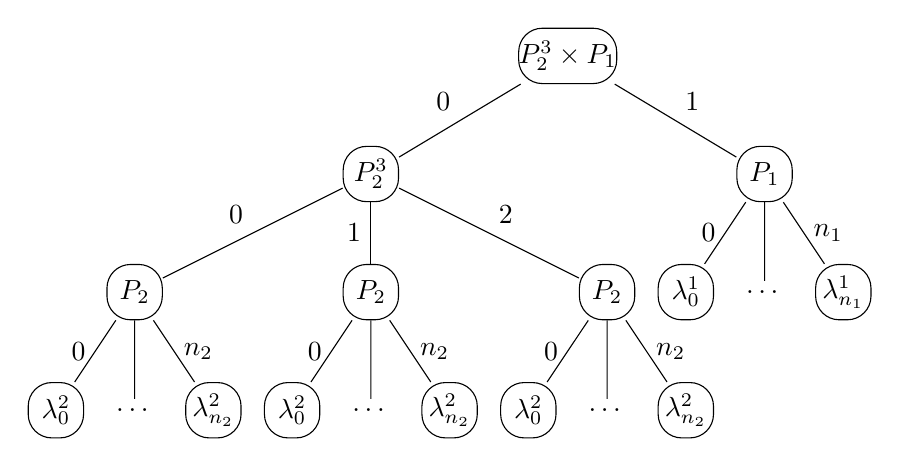
\begin{tikzpicture}[
                level/.style={
                    sibling distance = (3-#1)*2cm + 1cm,
                    level distance = 1.5cm
                }
            ]
            \node [treenode] {$P_2^3 \times P_1$}
                child{ node [treenode] {$P_2^3$}
                    child{ node [treenode] {$P_2$}
                        child{ node [basisnode] {$\lambda_0^2$} edge from parent node[left] {$0$}}
                        child{ node [] {$\dots$} }
                        child{ node [basisnode] {$\lambda_{n_2}^2$} edge from parent node[right] {$n_2$} }
                        edge from parent node[above left] {$0$}
                    }
                    child{ node [treenode] {$P_2$}
                        child{ node [basisnode] {$\lambda_0^2$} edge from parent node[left] {$0$}}
                        child{ node [] {$\dots$} }
                        child{ node [basisnode] {$\lambda_{n_2}^2$} edge from parent node[right] {$n_2$} }
                        edge from parent node[left] {$1$}
                    }
                    child { node [treenode] {$P_2$}
                        child{ node [basisnode] {$\lambda_0^2$} edge from parent node[left] {$0$}}
                        child{ node [] {$\dots$} }
                        child{ node [basisnode] {$\lambda_{n_2}^2$} edge from parent node[right] {$n_2$} }
                        edge from parent node[above right] {$2$}
                    }
                    edge from parent node[above left] {$0$}
                }
                child{ node [treenode] {$P_1$}
                    child [sibling distance=1cm] { node [basisnode] {$\lambda_0^1$} edge from parent node[left] {$0$} }
                    child [sibling distance=1cm] { node [] {$\dots$} }
                    child [sibling distance=1cm] { node [basisnode] {$\lambda_{n_1}^1$} edge from parent node[right] {$n_1$} }
                    edge from parent node[above right] {$1$}
                };
        \end{tikzpicture}
    \end{center}
    \caption{Index tree for Taylor--Hood with indices inherited from FE tree}
    \label{fig:dune_functions:taylor_hood_index_tree}
\end{figure}

This example already demonstrates two important requirements:
On the one hand natural multi-indices do not necessarily have
a fixed length.
On the other hand it shows that one may be interested to construct multi-indices
that do not mimic the structure of the finite element tree:
To increase data locality in assembled matrices for the Taylor--Hood basis it may be
preferable to group all velocity degrees of freedom corresponding to a single
$P_2$ basis function together, i.\,e., to use the index $[0,j,i]$
for the $j$-the $P_2$ basis function for the $i$-th component.
The corresponding alternative index tree is illustrated in
Figure~\ref{fig:dune_functions:taylor_hood_index_blocked_tree}.

\begin{figure}
    \begin{center}
        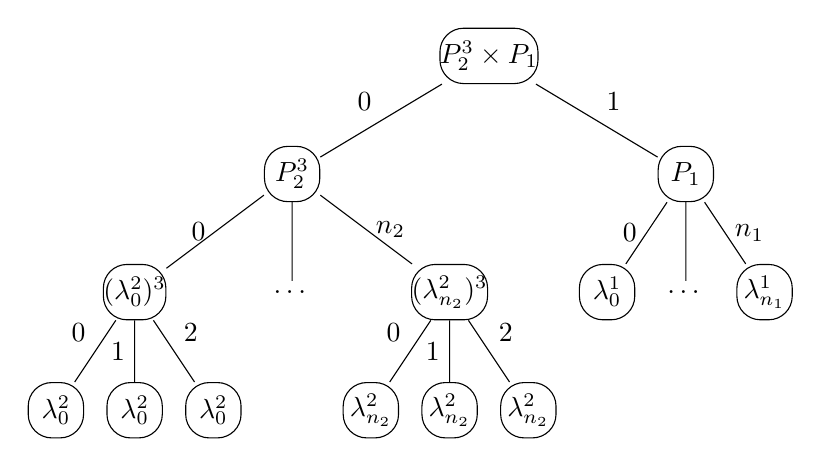
\begin{tikzpicture}[
                level/.style={
                    sibling distance = (3-#1)*2cm + 1cm,
                    level distance = 1.5cm
                },
            ]
            \node [treenode] {$P_2^3 \times P_1$}
                child{ node [treenode] {$P_2^3$}
                        child [sibling distance=2cm] { node [basisnode] {$(\lambda_0^2)^3$}
                            child{ node [treenode] {$\lambda_0^2$} edge from parent node[above left] {$0$}}
                            child{ node [treenode] {$\lambda_0^2$} edge from parent node[left] {$1$}}
                            child{ node [treenode] {$\lambda_0^2$} edge from parent node[above right] {$2$}}
                            edge from parent node[left] {$0$}
                        }
                        child [sibling distance=2cm]{ node [] {$\dots$} }
                        child [sibling distance=2cm]{ node [basisnode] {$(\lambda_{n_2}^2)^3$}
                            child{ node [treenode] {$\lambda_{n_2}^2$} edge from parent node[above left] {$0$}}
                            child{ node [treenode] {$\lambda_{n_2}^2$} edge from parent node[left] {$1$}}
                            child{ node [treenode] {$\lambda_{n_2}^2$} edge from parent node[above right] {$2$}}
                            edge from parent node[right] {$n_2$}
                        }
                        edge from parent node[above left] {$0$}
                }
                child{ node [treenode] {$P_1$}
                    child [sibling distance=1cm] { node [basisnode] {$\lambda_0^1$} edge from parent node[left] {$0$} }
                    child [sibling distance=1cm] { node [] {$\dots$} }
                    child [sibling distance=1cm] { node [basisnode] {$\lambda_{n_1}^1$} edge from parent node[right] {$n_1$} }
                    edge from parent node[above right] {$1$}
                };
        \end{tikzpicture}
    \end{center}
    \caption{Index tree for Taylor--Hood with blocking of local velocity components}
    \label{fig:dune_functions:taylor_hood_index_blocked_tree}
\end{figure}

To reflect this \dunemodule{dune-functions} essentially allows arbitrary
multi-indices as long as they are consistent in the sense that they
can be viewed as the paths to the leafs in an ordered tree.
%Consistency here means that the multi-indices should form an index tree.
That is, the children of each node are enumerated using consecutive zero-based
indices and paths to the leafs (i.e. the multi-indices) are build by concatenating
those indices starting from the root and ending in a leaf.
As motivated above, it is important to note, that this tree does not need to
coincide with the FE tree. A precise definition of such an index tree is given by
the following:

\begin{definition}
    \begin{enumerate}
        \item
            A tuple $I \in \N_0^k$ for some $k \in \N_0$ is called a multi-index of length $k$
            and we write $|I|=k$.
            The set of all multi-indices is denoted by
            $\mathcal{N} = \bigcup_{k \in \N_0^k} \N_0^k$.
        \item
            If $I \in \mathcal{N}$ takes the form $I = (I',I'')$ for $I',I'' \in \mathcal{N}$
            and $|I| = |I'|+|I''|$, then we call $I'$ a prefix of $I$ and write $I = (I',\dots)$.
            If additionally $|I''|>0$ we call $I'$ a strict prefix of $I$ and write $I = (I',*,\dots)$.
        \item
            A set $\mathcal{I} \subset \mathcal{N}$ is called an \emph{index tree}
            if for any $(I,i,\dots) \in \mathcal{I}$ there are also $(I,0,\dots),(I,1,\dots),\dots,(I,i,\dots) \in \mathcal{I}$
            but $I \notin \mathcal{I}$.
    \end{enumerate}
\end{definition}

If $\Lambda$ the set of basis functions of a finite element tree,
then \dunemodule{dune-functions} allows any indexing scheme that
is given by an index map $I: \Lambda \to \mathcal{N}$
whose range $I(\Lambda)$ is an index tree.

When operating with the indices of basis functions it is important
to know the maximal appearing index in order to allocate matrices
and vectors.
For a flat consecutive zero-based index this is just $d-1$ where
$d$ is the dimension of the spanned space. For multi-indices from
an index tree $\mathcal{I}$ we need a slightly more complicated
construction. Let $(I,\dots) \in \mathcal{I}$, i.\,e., $I$ is a
prefix of multi-indices in $\mathcal{I}$ then the size relative
to $I$ is given by
\begin{align*}
    |\mathcal{I}|_I = \op{max}\{k \st \exists (I,k,\dots) \in \mathcal{I} \}-1.
\end{align*}
In terms of the ordered tree associated with $\mathcal{I}$ this corresponds
to the number of direct children of the node indexed by $I$.


While \dunemodule{dune-functions} allows to use arbitrary index trees
to enumerate the basis functions, there are some important generic constructions
to derive such index trees from the finite element tree that will be described below.


\subsection{Ordering basis functions in a finite element basis tree}
\label{sec:dune_functions:basis_ordering}

To work with the basis of a finite element space, the basis vectors need to be indexed.  Indexing the basis functions
is what allows to address the corresponding vector and matrix coefficients in suitable vector and matrix data structures.
In simple cases, indexing means simply enumerating the basis functions with natural numbers, but for hierarchically
constructed spaces more general ways to index are possible.

There are two aspects to what we just have loosely called ``indexing''.  The first is that the set of all basis functions
in the tree need to be given a global order.  There are several reasonable choices to do this, which we discuss
in this section.
Given an order of the basis functions, there is then a natural indexing by simply enumerating the basis functions in
their specific order.
This is what we call the {\em flat} numbering, and very often this is what we want to use.  However, as the FE basis
is constructed hierarchically (and so may be the linear algebra data structures; see Chapter~\ref{sec:dune_istl:dune_istl}),
it may make sense to use hierarchical indices as well.  We discuss this in Section~\ref{sec:dune_functions:blocking}.

Consider first a leaf basis consisting of $n$ basis functions.  We suppose that these basis functions are given in a fixed
order (even though being able to change this ordering can improve the performance of a numerical
algorithm, see for example \cite{space_filling_curves,ordering_for_gauss_seidel} for more on this).
Consider now a tree of finite element bases with a given root $R$.  This root has $m$ children, and suppose that for
each of the subtrees rooted in these children we have already chosen an ordering.  Suppose further that the children themselves are given
in a fixed ordering (One may of course create different overall orderings by permuting the children, but in our view
this leads to a different bases, rather than to a different ordering of the same basis.)  It is then most natural
to first list all basis functions of the first tree, followed by all basis functions of the second subtree,
and so on.  This is the ordering obtained by a depth-first traversal of the tree~\cite{cormen:1990}.
For the Taylor--Hood basis with expression
\begin{equation*}
 B_\text{TH}
 =
 (B_x \otimes B_y \otimes B_z) \otimes B_p,
\end{equation*}
this means that the basis vectors are ordered as
\begin{equation*}
 b_{x,1}, b_{x,2}, \dots, b_{x,\abs{B_x}},
 b_{y,1}, \dots, b_{y,\abs{B_y}},
 b_{z,1}, \dots, b_{z,\abs{B_z}},
 b_{p,1}, \dots, b_{p,\abs{B_p}}.
\end{equation*}
(As this lists stands, but this has been done consciously to avoid overly technical notation.  Indeed, a given basis
function $b_{x,i}$ from the leaf basis is scalar valued.  However, in the product velocity space
$B_x \otimes B_y \otimes B_z$ the same basis function appears as $\mathbf{e}_1 b_{x,i} = (b_{x,i},0,0)^T$,
and now takes values in $\R^3$.  Furthermore, as part of the complete Taylor--Hood basis it is
$\tilde{\mathbf{e}}_1 b_{x,i} = (b_{x,i},0,0,0)^T$.  For the sake of the discussion here we identify a scalar
basis function $b_{x,i}$ with all of its vector-values variants.)

This is certainly a reasonable ordering.  Used in a finite element computation it will lead to a stiffness
matrix which, conceptually, consists of $4 \times 4$ large sparse blocks (Figure~\ref{fig:dune_functions:matrix_occupation_patterns}).
We call this the {\em lexicographic} ordering.

\begin{figure}
 \begin{center}
   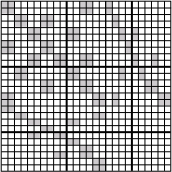
\includegraphics[width=0.4\textwidth]{taylor-hood-matrix-lexicographic}
   \qquad
   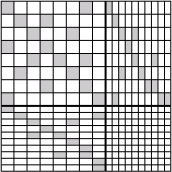
\includegraphics[width=0.4\textwidth]{taylor-hood-matrix-interleaved}
 \end{center}
 \caption{Two matrix occupation patterns.  Left: ordering the basis vectors of $B_x$, $B_y$, $B_z$, $B_p$
   one after the other gives a stiffness matrix with $4 \times 4$ sparse blocks.
   Right: interleaving the entries of $B_x$, $B_y$, $B_z$ gives a $2 \times 2$ block structure, where
   the entries are small blocks themselves.
   }
 \label{fig:dune_functions:matrix_occupation_patterns}
\end{figure}

However, there is one important alternative.  Since, for the standard applications of the Taylor--Hood element,
the $B_x$, $B_y$, $B_z$ bases are used to discretize the $x, y, z$ components of a velocity vector field,
it would be rather unusual not to use identical bases for these three coefficients.
In this case, all three bases have the same number of basis functions with the same ordering.  We can therefore
{\em interleave} the basis functions from the three subtrees.  That is,
the basis functions of the Taylor--Hood basis appear in the order
\begin{equation*}
 b_{x,1}, b_{y,1}, b_{z,1},
 b_{x,2}, b_{y,2}, b_{z,2},
 \dots
 b_{x,N}, b_{y,N}, b_{z,N},
 b_{p,1}, \dots, b_{p\abs{B_p}}.
\end{equation*}
In this case, the stiffness matrix only has $2 \times 2$ large sparse blocks, but each entry of the uppler left
block will be a $3 \times 3$ matrix, each entry of the lower right block will be a scalar, and the off-diagonal
blocks will have a corresponding rectangular structure (Figure~\ref{fig:dune_functions:matrix_occupation_patterns}).

To deduce such possibilities from the tree structure we now divide the inner tree nodes into two classes.
An inner node will be called {\em power node}, if all of its children are identical subtrees.
An inner node that is not a power node is called {\em composite node}.  To construct an admissible ordering
of all basis functions in a tree we move recursively from the leaf nodes to the root.  To start the recursion,
the order of the basis functions in each leaf node is considered fixed.  At each inner node there are two
possibilities.
\begin{enumerate}
 \item The inner node is a composite node.  Then the basis functions of all the subtrees (with the ordering
   within each subtree already given by recursion) are concatenated to obtain lexicographic ordering.
   Remember that we suppose the order of the children to be fixed.
 %
 \item The inner node is a power node.  Then there are two choices: Either combine the subtree basis functions
   in lexicographic order, or interleave them.
\end{enumerate}
In total, for a tree with $N$ power nodes we obtain $2^N$ different ways to order the basis functions of the tree.



\subsection{Grouping degrees of freedom in blocks}
\label{sec:dune_functions:blocking}

So far we have not mentioned what what we mean by ``index''.  Certainly it is possible to assign the numbers
$1, \dots, n$ to the basis vectors of an $n$-dimensional space.  However, such a {\em flat} numbering discards
quite a bit of information about the structure of the space.
\begin{enumerate}
 \item Even though stiffness matrices may have a very specific occupation pattern (such as the blocked
   Taylor--Hood example in Figure~\ref{fig:dune_functions:matrix_occupation_patterns}), it is very difficult
   to use in a data structure.  For example, quite a lot of memory can be saved if that matrix data
   structure knows that its entries are grouped in little $3 \times 3$ blocks.
 %
 \item Likewise, the solver can be more efficient when the structure of the matrix is known to it.
   For example, block variants are frequently more efficient.
 %
 \item Finally, it can ease debugging if the structure of the finite element space is (partially)
   contained in the number type.
\end{enumerate}
For these reasons, \dunemodule{dune-functions} uses multi-indices instead of natural numbers to index
its global degrees of freedom.
\todo[inline]{Erklären: Wie kommt man vom Baum zum Multi-Index}
Even for a fixed global ordering of the basis functions of a finite element tree, there is usually more
than one way to address the individual basis functions using multi-indices.  Just like for the orderings
the different ways to construct multi-indices can be read off from the tree structure.%
%
\footnote{Note how using a multi-index to address basis functions partitions the basis functions into
separate blocks.  For example, if a two-digit multi-index is used, all basis functions with first digit $0$
form one block.  Therefore we sometimes speak of ``blocking'' of basis functions when their assignment
to certain multi-indices is meant.}

\todo[inline, caption={}]
{
  Jetzt haben wir ein Problem.  Man will Multi-Indizes auch für ein paar Unterscheidungen haben, die nicht
  in der Baumstruktur auftauchen, z.B.
  \begin{itemize}
   \item Elementblöcke bei DG-Verfahren
   \item Unterscheidung der Freiheitsgrade nach Entities / Hierarchische Basen
   \item XFEM
  \end{itemize}
 Problem: Das sind alles {\em additive} Zerlegungen des Raums, und die sind bisher in \dunemodule{dune-functions}
 nicht offiziell vorgesehen.
}

Instead of flat integers, we therefore use a hierarchical numbering scheme that reflects the tree structure
of the space.  Instead of integer numbers we obtain multi-indices, i.e., certain tuples.
Consider a tree representing a finite element space like for example the tree for the Taylor--Hood space in
Figure~\ref{fig:dune_functions:taylor_hood_basis_tree}.

We construct multi-indices for this tree by recursion over the tree depth.  To start the recursion,
we suppose that each ``simple'' (leaf) basis provides a numbering of its basis vectors.  This numbering is
a flat numbering of all basis vectors, using a single integer.

Multi-indices for the basis vectors represented by subtrees are now defined recursively.  Let $R$ be the tree root
of a subtree of the finite element basis tree, and suppose that we can already construct multi-indices
for all basis vectors of its children.  Then we construct multi-indices for the vectors of $R$ itself
by first numbering all children of $R$ by a number $0,\dots,n_R-1$.  A vector $b$ in the basis of the
subtree of $R$ is then constructed by prepending the number of the corresponding child node to the
multi-index of $b$ in that child.

\todo[inline]{Hier sind wir bisher noch unsauber: wenn $b$ ein Vektor aus einer Blatt-Basis ist,
so ist er kein Vektor eines inneren Knoten.}

\begin{itemize}
 \item Note that not all multi-indices have the same size
\end{itemize}


\begin{table}
 \begin{center}
 \begin{tabular}{c|c|c|c|c}
 \hline \\
  $b_{x,0}$  & $0$    & $(0,0)$ & $(0,0)$ & $(0,0,0)$ \\
  $b_{x,1}$  & $1$    & $(0,1)$ & $(0,1)$ & $(0,0,1)$ \\
  $b_{x,2}$  & $2$    & $(0,2)$ & $(0,2)$ & $(0,0,2)$ \\
    \vdots   & \vdots & \vdots  & \vdots  & \vdots  \\
  $b_{y,0}$  & $n$    & $(0,n)$ & $(1,0)$ & $(0,1,0)$ \\
  $b_{y,1}$  & $n+1$  & $(0,n+1)$ & $(1,1)$ & $(0,1,1)$ \\
  $b_{y,2}$  & $n+2$  & $(0,n+2)$ & $(1,2)$ & $(0,1,2)$ \\
    \vdots   & \vdots & \vdots  & \vdots  & \vdots  \\
  $b_{z,0}$  & $2n$   & $(0,2n)$ & $(2,0)$ & $(0,2,0)$ \\
  $b_{z,1}$  & $2n+1$ & $(0,2n+1)$ & $(2,1)$ & $(0,2,1)$ \\
  $b_{z,2}$  & $2n+2$ & $(0,2n+2)$ & $(2,2)$ & $(0,2,2)$ \\
    \vdots   & \vdots & \vdots  & \vdots  & \vdots  \\
  $p_0$      & $3n$   & $(1,0)$ & $n$ & $(1,0)$ \\
  $p_1$      & $3n+1$ & $(1,1)$ & $n+1$ & $(1,1)$ \\
  $p_2$      & $3n+2$ & $(1,2)$ & $n+2$ & $(1,2)$ \\
    \vdots   & \vdots & \vdots  & \vdots  & \vdots
 \end{tabular}
 \end{center}
 \caption{Possible index types for a Taylor--Hood basis with lexicographic ordering of the velocity basis functions}
 \label{tbl:dune_functions:th_multiindices_lexicographic}
\end{table}

\begin{table}
 \begin{center}
 \begin{tabular}{c|c|c|c|c}
 \hline \\
  $b_{x,0}$  & $0$    & $(0,0)$ & $(0,0)$ & $(0,0,0)$ \\
  $b_{y,0}$  & $1$    & $(0,1)$ & $(0,1)$ & $(0,0,1)$ \\
  $b_{z,0}$  & $2$    & $(0,2)$ & $(0,2)$ & $(0,0,2)$ \\
  $b_{x,1}$  & $3$    & $(0,3)$ & $(1,0)$ & $(0,1,0)$ \\
  $b_{y,1}$  & $4$    & $(0,4)$ & $(1,1)$ & $(0,1,1)$ \\
  $b_{z,1}$  & $5$    & $(0,5)$ & $(1,2)$ & $(0,1,2)$ \\
  $b_{x,2}$  & $6$    & $(0,6)$ & $(2,0)$ & $(0,2,0)$ \\
  $b_{y,2}$  & $7$    & $(0,7)$ & $(2,1)$ & $(0,2,1)$ \\
  $b_{z,2}$  & $8$    & $(0,8)$ & $(2,2)$ & $(0,2,2)$ \\
    \vdots   & \vdots & \vdots  & \vdots  & \vdots  \\
  $p_0$      & $3n$   & $(1,0)$ & $n$ & $(1,0)$ \\
  $p_1$      & $3n+1$ & $(1,1)$ & $n+1$ & $(1,1)$ \\
  $p_2$      & $3n+2$ & $(1,2)$ & $n+2$ & $(1,2)$ \\
    \vdots   & \vdots & \vdots  & \vdots  & \vdots
 \end{tabular}
 \end{center}
 \caption{Possible index types for a Taylor--Hood basis with interleaved ordering of the velocity basis functions
 \todo[inline]{Inkonsistenz:  Der Index in der rechten Spalte ist so wie man ihn als Programmierer erwarten würde.
   Aus Sicht der Baumkonstruktion ist er allerdings inkonsequent.  Der skalare Index in einer einzelnen Blatt-Basis
    erscheint nicht als letzte Stelle im Multi-Index, sondern als {\em vorletzte}.  Das muss man ordentlich
    begründen, und schauen was in allgemeineren Bäumen passiert.}
 \label{tbl:dune_functions:th_multiindices_interleaved}
 }
\end{table}



\section{Programmer interface for function space bases}
\label{sec:dune_functions:function_space_bases_implementation}

The design of the \dunemodule{dune-functions} interfaces for bases of discrete function spaces
follows the ideas of the previous section.  In a nutshell, a \dunemodule{dune-functions} function space basis
does two things for you: For each element it gives you access to the (tree of) shape functions there,
and it provides the mapping from element-local shape function numbers to global basis function numbers.

\begin{figure}
 \begin{center}
  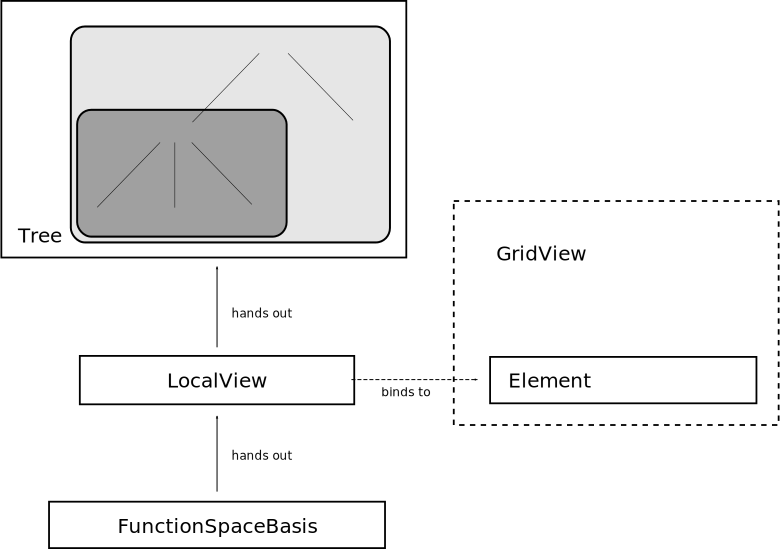
\includegraphics[width=\textwidth]{febasis_interface_schematic}
 \end{center}
 \caption{Overview of the classes making up the interface to finite element space bases}
 \label{fig:dune_functions:febasis_interface_schematic}
\end{figure}


To reflect this, the interface of function space bases is divided into two parts.  A \cpp{LocalView} on an
element allows you to obtain the finite element of that element, which in turn gives you access to all
shape functions, associations to element subentities, and local interpolation rules provided by
\dunemodule{dune-localfunctions}.  The mapping of these shape functions to global degrees of freedom is
delegated to a separate object called a \cpp{LocalIndexSet}, which you can bind to given
\cpp{LocalView} objects.  Once bound, a \cpp{LocalIndexSet} will provide global (multi-)indices
for each shape function on this element.  The structure of the interface is visualized in
Figure~\ref{fig:dune_functions:febasis_interface_schematic}.

\subsection{Function space bases defined on a grid view}

The basis interface is implemented in a mix of static and dynamic polymorphism.  For each concept
there is a pure abstract base class in \file{dune/functions/functionspacebases/gridviewfunctionspacebasis.hh},
and implementations of function space bases should inherit from these classes.  On the other hand,
objects are usually handed out by-value, and so the classes can be used in a statically polymorphic
context.

Main interface class is the class \cpp{GridViewFunctionSpaceBasis}, which represents a basis of a
function space defined on a single grid view.%
\footnote{As opposed to, say, a basis defined only on parts of a grid view.}
The class is declared in
\file{dune/functions/functionspacebases/gridviewfunctionspacebasis.hh}.  The interface of this class
is fairly short.  Table~\ref{} lists the exported static information,
and Table~\ref{} lists all public methods.
As you can see, the class takes four template parameters, which all represent types.  They are
\begin{description}
 \item [GV] The grid view (i.e., non-hierarchical grid) that the basis is defined on,
 \item [LV] the type implementing the restriction of the basis to a single element,
 \item [IS] the type implementing the basis index set,
 \item [MI] The type used for multi-indices.
\end{description}
These types are exported by the interface class as \cpp{GridView}, \cpp{LocalView}, \cpp{IndexSet}, and
\cpp{MultiIndex}, respectively.  The class has four public methods, all of which are \cpp{const}
and pure virtual.  The method \cpp{gridView} returns the grid view object that the basis is
defined on.  The method \cpp{localIndexSet} returns the index set object, which we discuss below.

Finally, the main method is called \cpp{localView}.  It returns the restriction of the basis
to a single element.  This restriction then provides access to the actual shape functions and
their numbers.  Note that the method \cpp{localView} does not take any arguments.

\subsection{\texorpdfstring{\cpp{LocalView}}{LocalView} objects and the tree of shape functions}

The \cpp{localView}
method produces a \cpp{LocalView} object that is {\em free}, i.e., not associated to any
element of the grid view.  Before being useful it needs to be bound to a particular element.

The interface of the \cpp{LocalView} class is again rather short.  Tables~\ref{}
and~\ref{} list the exported static data and the public methods, respectively.
The \cpp{bind} method accepts a grid element and binds the view to the element.  Nothing can be done with a
\cpp{LocalView} object before it is bound to an element.  This construction allows to perform element-related
setup tasks once in the \cpp{bind}-method, and obtain faster calls afterwards.

Once the view is bound to an element, you can obtain the tree of finite elements by calling the \cpp{tree}
method.  The resulting object is a tree as described in Chapter~\ref{}.

Trees are constructed from three parts, corresponding to Chapter~\ref{}.
Leaf nodes implement scalar local finite elements.  Power nodes are inner tree nodes that combine a number
of identical subtrees.  Finally, composite nodes combine non-identical subtrees.  Each of the three classes
has an interface class, and we discuss each of them in turn.  If all you are interested in are
scalar finite elements, you only have to read about the leaf nodes.

\begin{itemize}
 \item Leaf nodes
 \item Power nodes
 \item Composite nodes
 \item localIndex method
\end{itemize}

\begin{description}
\item[CompositeBasis] A \cpp{CompositeBasis} is the product of an arbitrary collection of underlying bases and is the
most versatile representation of a composite space. We will use this class to create the overall space $V_{TH}$.
The corresponding C++ class simply takes the list of components as both template and constructor parameters:
\begin{lstlisting}
template<typename... Components>
class CompositeBasis
{
  ...
  // Construct a CompositeBasis from its components
  CompositeBasis(Components&&... components);

  // Equivalent interface for dynamically allocated components
  CompositeBasis(shared_ptr<Components>... component_pointers);
  ...
};
\end{lstlisting}
\item[PowerBasis] While the \cpp/CompositeBasis/ can be used for any kind of product space, it may not always be the most natural
or efficient model for it. Our velocity space is a good example for this: We can most naturally understand it as a vector-valued
version of the underlying scalar space $V_v = (P_2)^3$. The \cpp/PowerBasis/ is a direct model of this concept and describes
a composite space as a combination of a single component space and an integer power $k$:
  \begin{lstlisting}
template<typename Component, std::size_t k>
class PowerBasis
{
  ...
  // This constructor will duplicate its argument k times
  PowerBasis(Component&& component);
  // This constructor requires exactly k arguments and should be used
  // if the components have to be set up individually
  PowerBasis(Component&... components);

  // Equivalent interface for dynamically allocated components
  PowerBasis(shared_ptr<Component> component_pointer);
  PowerBasis(shared_ptr<Component>... component_pointers);
  ...
};
  \end{lstlisting}
\end{description}


\subsection{Global shape function indices}

The basis functions of this tree are numbered, and these numbers are what you use to index rows and columns
of your element stiffness matrix.  As explained in Chapter~\ref{sec:dune_functions:basis_ordering}, there is a range
of possibilities to index the basis functions in a finite element tree.  However, for this element-local
tree, only the flat index is available.  It is our (current) belief that only this
index is needed for indexing local basis functions, and providing no alternative reduces interface
complexity considerably.  On the other hand, for the indexing of the global basis functions, having the choice
between different numberings is definitely useful.

Consider, for example, a $k$-th order DG space on a triangle grid.  It is always reasonable to use a normal
random access container such as \cpp{std::vector<double>} to store coefficients of finite element functions.
Such containers are indexed with a flat index.


\subsection{Function space bases available in \texorpdfstring{\dunemodule{dune-functions}}{dune-functions}}

The \dunemodule{dune-functions} module contains a collection of finite element bases that implement
this interface.  At the time of writing these are:

\begin{itemize}
 \item \cpp{PQkNodalBasis}: Lagrangian bases of order $k$, where $k$ is a compile-time parameter.
   For $k\le 2$, this implementation works on all kinds of conforming grids, including grids with more
   than one element type.  At the time of writing, higher-order spaces are implemented only partially.
   Check the online class documentation for the current status.

 \item \cpp{PQ1NodalBasis}: Lagrangian nodal bases of first order.  This is a separate implementation of
   the case $k=1$ of the previous basis.  It exists mainly so that people interested in writing their
   own bases have a simple example to look at.

 \item \cpp{TaylorHoodBasis}: The Taylor--Hood bases described in Chapter~\ref{sec:dune_functions:finite_element_trees}.
   This is a simple example of basis constructed by building products.
   A complete example for how to use this basis is given in Chapter~\ref{sec:stokes_example}.

 \item \cpp{LagrangeDGBasis}: Implements a $k$-th order Discontinuous-Galerkin basis with Lagrange shape functions.
   The shape functions are the same as for the \cpp{PQkNodalBasis},
   but the basis functions are not continuous across the element boundaries.  Therefore, this basis also
   works well on non-conforming grids.  The polynomial order is again a compile-time constant.

 \item \cpp{BSplineBasis}:  Implements a $B$-Spline basis on a structured, axis-aligned grid as described,
   e.g., in~\cite{cottrell_hughes_bazilevs:2009}.  Arbritrary orders, dimensions, and knot vectors are supported,
   allowing, e.g., to work with $C^1$ elements for fourth-order differential equations.

   Each \cpp{BSplineBasis} object implements a basis on a single patch, and the grid must correspond to this
   patch. For this to work, several restrictions apply for the grid.  It must be structured and axis-aligned,
   and consist of (hyper-)cube elements only.  Further, the element indices must be lexicographic and
   increase from the lower left to the upper right domain corner.  The element spacing must math the knot spans.
   Unfortunately, not all these requirements can be checked for by the basis, so users have to be a bit
   careful.  Using a \cpp{YaspGrid} object works well.

   Note that unlike in standard finite element bases, in a B-spline basis basis functions cannot be associated
   to grid entities such as vertices, edges, or elements.  The interface nevertheless mandates that a
   \cpp{LocalCoefficient} object must be available, but for the \cpp{BSplineBasis}, the behavior of this
   object is undefined.
\end{itemize}



\section{Solving the Stokes equation with \dunemodule{dune-functions}}
\label{sec:stokes_example}

\subsection{The Stokes equation}

\begin{figure}
 \begin{center}
  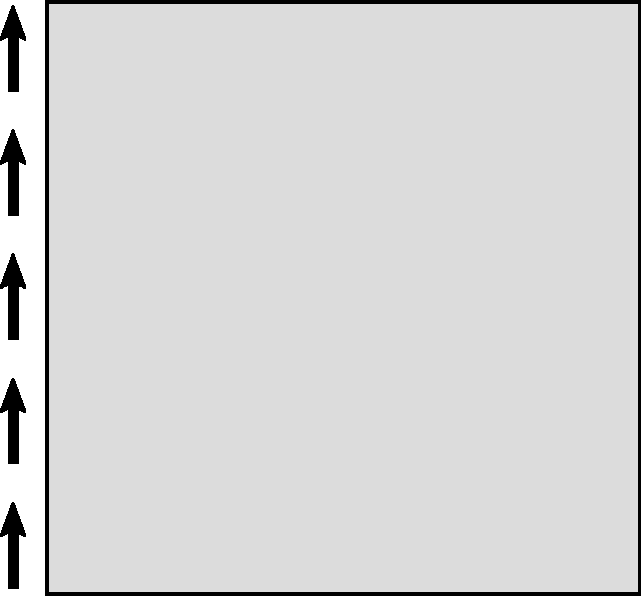
\includegraphics[height=0.3\textheight]{driven_cavity}
  \qquad
  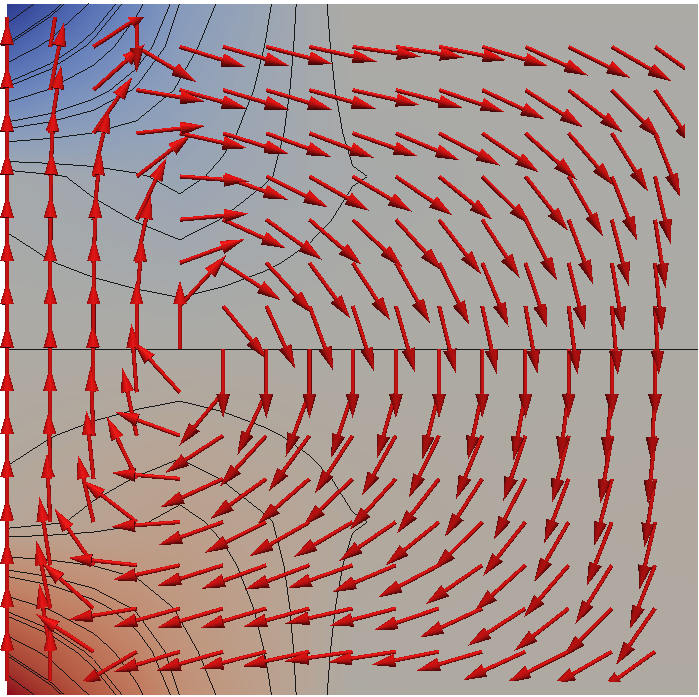
\includegraphics[height=0.3\textheight]{driven_cavity_result}
 \end{center}
 \caption{Driven cavity. Left: setting, right: simulation result.  The arrows show the {\em normalized} velocity.}
 \label{fig:dune_functions:driven_cavity}
\end{figure}

The Stokes equation models a viscous incompressible
fluid in a $d$-dimensional domain $\Omega$.  There are two unknowns in this problem: a stationary
fluid velocity field $\mathbf{u} : \Omega \to \R^d$, and the fluid pressure $p : \Omega \to \R$.
Together, they have to solve the boundary value problem
\begin{alignat*}{2}
 -\Delta \mathbf{u} - \nabla p & = 0  & \qquad & \text{in $\Omega$} \\
 \div \mathbf{u} & = 0                &        & \text{in $\Omega$} \\
                    \mathbf{u} & = \mathbf{u}_D  &        & \text{on $\partial \Omega$},
\end{alignat*}
where we have omitted the physical parameters.  The boundary value problem only determines the
pressure $p$ up to a constant function.  The pressure is therefore usually normalized such
that $\int_\Omega p\,dx = 0$.

Due to the constraint $\div \mathbf{u} = 0$, the corresponding weak form of the equation is a saddle-point problem.
Introduce the spaces
\begin{align*}
 \mathbf{H}^1_D(\Omega)
      & \colonequals
      \big\{ \mathbf{v} \in \mathbf{H}^1(\Omega) \; :\; \operatorname{tr}{\mathbf{v}} = \mathbf{u}_D \big\}, \\
 L_{2,0}(\Omega) & \colonequals  \Big\{ q \in L_2(\Omega) \; :\; \int_\Omega q\,dx = 0 \Big\},
\end{align*}
and the bilinear forms
\begin{equation*}
 a(\mathbf{u},\mathbf{v}) \colonequals \int_\Omega \nabla \mathbf{u} \nabla \mathbf{v} \,dx,
 \qquad \text{and} \qquad
 b(\mathbf{v},q) \colonequals \int_\Omega \div \mathbf{v} \cdot q \,dx.
\end{equation*}
Then the weak form of the Stokes equation is: Find $(\mathbf{u},p) \in \mathbf{H}_D^1(\Omega) \times L_{2,0}(\Omega)$ such that
\begin{alignat*}{2}
 a(\mathbf{u},\mathbf{v}) + b(\mathbf{v},p) & = 0 & \qquad & \text{for all $\mathbf{v} \in \mathbf{H}_0^1(\Omega)$} \\
 b(\mathbf{u},q)\qquad\qquad & = 0       &        & \text{for all $q \in L_{2,0}(\Omega)$}.
\end{alignat*}
If $\mathbf{u}_D$ is sufficiently smooth, this variational problem has a unique solution.
The Taylor--Hood element is the standard way to discretize this saddle point problem~\cite{braess:2013}.

\subsection{The driven-cavity benchmark}

For our example we choose to simulate a two-dimensional driven cavity.  This is a standard benchmark
for the Stokes problem in the literature.  Let $\Omega$ be the unit square $[0,1]^2$, and set the Dirichlet
boundary conditions for the velocity $\mathbf{u}$ to
\begin{equation*}
 \mathbf{u}(x)
 =
 \begin{cases}
  (0,1) & \text{if $x \in \{0\} \times [0,1]$} \\
  (0,0) & \text{elsewhere on $\partial \Omega$}.
 \end{cases}
\end{equation*}
The interpretation of this is a fluid container that is closed on all but one side.  While the fluid remains
motionless on the closed sides, an external agent drives a constant upward motion on the left vertical side.
The domain and boundary conditions are depicted in Figure~\ref{fig:dune_functions:driven_cavity}, left.
The corresponding solution is shown on the right side of the same figure.  The velocity forms a vortex,
while the pressure forms extrema in the two left corners.

In the following discussion we always use the letter $d$ to denote the space dimension, even though it is
known to be $d=2$ for our specific example.  This is to avoid confusion, because the number~2 also
appears a few times because we have two types of unknowns.

\subsection{Discretization}

\begin{figure}
  \begin{center}
   \begin{overpic}[width=0.5\textwidth]{taylor_hood_tree}
    \put(5,5){$P_2$}
    \put(30,5){$P_2$}
    \put(55,5){$P_2$}
    \put(87,31){$P_1$}
    \put(5,30){$V_\text{v}$}
    \put(5,57){$B_\text{TH}$}
    \put(30.7,32){$\otimes$}
    \put(61.6,58){$\otimes$}
   \end{overpic}

  \end{center}
  \caption{Taylor--Hood basis $P_2 \otimes P_2 \otimes P_2 \otimes P_1$ in a tree representation}
    \label{fig:taylor_hood_basis_tree}
\end{figure}

We discretize the domain using a structured axis-aligned grid with $4 \times 4$ uniform quadrilateral elements.
On this grid, we use the Taylor--Hood element to discretize the weak saddle-point problem.  The nodal basis
of the Taylor--Hood element has a natural tree structure as shown in Figure~\ref{fig:taylor_hood_basis_tree}.
On each element, the \dunemodule{dune-functions} implementation provides a local numbering of all shape functions
on this element.  This numbering uses a simple integer as index type, and is used to address the entries of the
element stiffness matrix.

\begin{table}
 \begin{center}
 \begin{tabular}{c|c}
 basis function & multi-index \\
 \hline \\
  $b_{x,0}$  & $(0,0)$ \\
  $b_{y,0}$  & $(0,1)$ \\
  $b_{z,0}$  & $(0,2)$ \\
  $b_{x,1}$  & $(0,3)$ \\
  $b_{y,1}$  & $(0,4)$ \\
  $b_{z,1}$  & $(0,5)$ \\
  $b_{x,2}$  & $(0,6)$ \\
  $b_{y,2}$  & $(0,7)$ \\
  $b_{z,2}$  & $(0,8)$ \\
    \vdots   & \vdots  \\
  $p_0$      & $(1,0)$ \\
  $p_1$      & $(1,1)$ \\
  $p_2$      & $(1,2)$ \\
    \vdots   & \vdots
 \end{tabular}
 \end{center}
 \caption{Multi-index for the Taylor--Hood basis with interleaved ordering of the velocity basis functions}
 \label{tbl:th_multiindices_interleaved}
\end{table}

Each global basis function additionally gets a global index, used to address the entries of the global stiffness
matrix.  In principle, \dunemodule{dune-functions} provides several types of orderings and multi-indices here.
The one that is used in the code example is given  in Table~\ref{tbl:th_multiindices_interleaved}: Each global
index is a pair $(a,b)$, where $a \in \{0,1\}$ switches between velocity and pressure basis functions,
and $b \in \mathbb{N}$ selects a particular basis function in either the set of velocity basis functions
or the set of pressure basis functions.


\subsection{Implementation}

This chapter discusses an example implementation of the Stokes problem, using only \dunemodule{dune-functions}
and no higher-level modules.  The example is contained in a single file, which comes as part of the \dunemodule{dune-functions}
source tree, in \file{dune-functions/examples/stokes-taylorhood.cc}.  If you read this document in electronic form,
the file can also be accessed by clicking on the icon in the margin.%
%
\marginpar{\attachfile[author=The dune-functions team,
                       color = 1 0 0,
                       mimetype=text/plain,
                       description=Complete source code of the Stokes/Taylor-Hood example]
                       {../../examples/stokes-taylorhood.cc}}

\subsubsection{The \texorpdfstring{\cpp{main}}{main} method}

We begin discussing the example code by describing its \cpp{main} method.  This method begins by setting up MPI and the grid.
We pick \cpp{YaspGrid} for the structured $4 \times 4$ quadrilateral grid.  Note that there is the line
%
\lstinputlisting[linerange={using_namespace_dune_begin-using_namespace_dune_end},
                 numbers=left]{../../examples/stokes-taylorhood.cc}
%
at the top of the file, so this namespace is imported completely.  Additionally, everything in the \dunemodule{dune-functions}
module is in the namespace \cpp{Functions}.  This namespace is not imported; instead, the prefix \cpp{Functions::} is always
given explicitly.


%
\lstinputlisting[linerange={main_begin-grid_setup_end},
                 numbers=left]{../../examples/stokes-taylorhood.cc}
%
The \cpp{gridView} object is the flat finite element grid that we will use for
the computation.
On this grid view, we then set up the function space basis for the Taylor--Hood element.  This is as simple as
%
\lstinputlisting[linerange={function_space_basis_begin-function_space_basis_end},
                 numbers=left]{../../examples/stokes-taylorhood.cc}
%
For each element, the \cpp{taylorHoodBasis} object will give us the tree of shape functions, and the corresponding local and global numberings.

Before being able to assemble the stiffness matrix of the Stokes system we need to pick suitable data structures
for the linear algebra.
The implementation of the Taylor--Hood basis selected in Line~\ref{li:stokes_taylorhood_select_taylorhoodbasis} orders the
velocity degrees of freedom before the pressure degrees of freedom.  Further, the velocity
components are interleaved.  The indexing scheme results from grouping degrees of freedom at the
tree root.  The resulting multi-indices all have length~2, and are given in Table~\ref{tbl:th_multiindices_interleaved}.
Consequently, the appropriate vector type is a pair of scalar vectors, one for the velocity and one for the pressure
degrees of freedom.  Analogously, the matrix must consist of $2 \times 2$ large sparse scalar matrices.
The following code sets up vector and matrix types for this, using the nesting machinery from \dunemodule{dune-istl}.
%
\lstinputlisting[linerange={linear_algebra_setup_begin-linear_algebra_setup_end},
                 numbers=left]{../../examples/stokes-taylorhood.cc}
%
Other index types are possible and possibly desirable here.  These would correspond to other vector and
matrix data types.

Now that we have chosen the C++ types for the matrix and vector data structures we can actually assemble the system.
Assembling the right-hand-side vector \cpp{rhs} is easy, because, apart from the Dirichlet boundary data (which we
will insert later), all its entries are zero.  An all-zero vector of the correct type and size is set up by the
following lines
%
\lstinputlisting[linerange={rhs_assembly_begin-rhs_assembly_end},
                 numbers=left]{../../examples/stokes-taylorhood.cc}
%
The \cpp{HierarchicVectorView} is a device that offers easier handling of arbitrarily nested vector data types.
In particular, it offers convenient resizing of an entire hierarchy of nested vectors.
The \cpp{taylorHoodBasis} object informs about the sizes of the corresponding finite element basis subtrees,
and Line~\ref{li:stokes_taylorhood_set_rhs_to_zero} fills the entire vector with zeros.

To obtain the stiffness matrix we first create an empty matrix object of the correct type.  The actual assembly
is factored out into a separate method.
%
\lstinputlisting[linerange={matrix_assembly_begin-matrix_assembly_end},
                 numbers=left]{../../examples/stokes-taylorhood.cc}
%
As the matrix assembly is the central part of this example we explain it in detail below, after having covered the \cpp{main} method.

Suppose now that we have the correct stiffness matrix assembled in the object \cpp{stiffnessMatrix}.  We still need
to modify the linear system to include the Dirichlet information.
In a first step we need to determine all degrees of freedom with Dirichlet data.  These are all the velocity degrees of freedom
on the domain boundary.  We could do this by using the \cpp{LocalKey} object of each basis function
to single out all those that are assigned to a boundary entity.  However, on a simple domain as the unit square
used here it is easier to use a geometric criterion.  We first define a predicate that returns \cpp{true}
if a given global coordinate \cpp{x} is on the domain boundary:
%
\lstinputlisting[linerange={boundary_predicate_begin-boundary_predicate_end},
                 numbers=left]{../../examples/stokes-taylorhood.cc}
%
The we interpolate this boolean-valued function in the space spanned by the velocity basis functions.
%
\lstinputlisting[linerange={interpolate_boundary_predicate_begin-interpolate_boundary_predicate_end},
                 numbers=left]{../../examples/stokes-taylorhood.cc}
%
Observe how the \dunemodule{dune-functions} interface allows to interpolate C++11 lambdas, which makes the code
very short and readable.  The expression \cpp{TypeTree::hybridTreePath(_0,i)} selects the different coordinate
directions of the velocity basis from the tree representation given in Figure~\ref{fig:taylor_hood_basis_tree}.
As the bases for the velocity components are all the same, an ordinary integer \cpp{i} is sufficient to choose
one of them.  In contrast, the velocity and pressure bases are different C++ types, and a compile-time
construction is needed to choose between them.  The object \cpp{_0} is defined in
\file{dune/typetree/utility.hh} as (roughly)
\begin{lstlisting}
std::integer_constant<std::size_t, 0> _0;
\end{lstlisting}
In the \cpp{TaylorHoodBasis} implementation, \cpp{_0} selects the velocity subtree and \cpp{_1} selects
the pressure subtree.

Finally, we define a function implementing the actual Dirichlet values function $\mathbf{u}_D$, and interpolate
that into the right-hand-side vector \cpp{rhs}.
%
\lstinputlisting[linerange={interpolate_dirichlet_values_begin-interpolate_dirichlet_values_end},
                 numbers=left]{../../examples/stokes-taylorhood.cc}
%
The expression \cpp{TypeTree::hybridTreePath(_0)} demands that only velocity degrees of freedom are
interpolated.  The \cpp{isBoundary} vector given as the last argument restricts the interpolation
to only the boundary degrees of freedom.

The stiffness matrix is modified in a more manual fashion.  For each Dirichlet degree of freedom we need to fill the corresponding matrix row
with zeros, and write a~1 on the diagonal.  As only velocity
degrees of freedom have Dirichlet values, we need to modify the two upper matrix blocks only.
%
\lstinputlisting[linerange={set_dirichlet_matrix_begin-set_dirichlet_matrix_end},
                 numbers=left]{../../examples/stokes-taylorhood.cc}
%
Finally, we can solve the linear system.  Efficiently solving the Stokes system is an art, which we do not want to
get into here.  Instead, we a GMRes solver, without any preconditioner at all.  This is known to converge,
albeit slowly.
\todo[inline]{Eigentlich peinlich.  Können wir nicht doch einen vernünftigen Löser nehmen?}
The advantage is that it can be written down in very few lines.
%
\lstinputlisting[linerange={stokes_solve_begin-stokes_solve_end},
                 numbers=left]{../../examples/stokes-taylorhood.cc}
%
Observe how the \cpp{RestartedGMResSolver} object is completely oblivious to the fact that the matrix
has a two-level nesting structure.  On the other hand, dedicated Stokes solvers usually operate
on some sort of Schur complement, and hence they need direct access
to the four submatrices.  This can be elegantly done using the nested matrix type
used for the stiffness matrix.

Once the iterative solver has terminated, we write the result to a VTK file.  For this, we write the resulting velocity as a vector field,
and the resulting pressure as a scalar field.  We subsample the grid twice, because the \cpp{VTKWriter}
class natively only displays piecewise linear functions.
%
\lstinputlisting[linerange={stokes_output_begin-stokes_output_end},
                 numbers=left]{../../examples/stokes-taylorhood.cc}
%
When run, this program produces a file called \file{function-stokes-result.vtu}.  The file can be opened in
\program{ParaView}, and the outcome looks like the image on the right in Figure~\ref{fig:dune_functions:driven_cavity}.

\subsubsection{The global assembler}

Now that we have covered the \cpp{main} method, we can turn to the assembler for the Stokes stiffness matrix.
As our main focus is the use of the \dunemodule{dune-functions} interfaces, the assembler
is the central part of our example.   We begin with the global assembler,
which is the routine \cpp{assembleStokesMatrix} called in Line~\ref{li:stokes_taylorhood_call_to_assemblestokesmatrix}
of the \cpp{main} method.
The global assembler sets up the matrix pattern, loops over all elements, and accumulates the element stiffness
matrices in the global matrix. The signature of the method is
%
\lstinputlisting[linerange={global_assembler_signature_begin-global_assembler_signature_end},
                 numbers=left]{../../examples/stokes-taylorhood.cc}
%
The only arguments it gets are the finite element basis and the matrix to fill.  Observe that the Taylor--Hood basis is not
hard-wired here, so we could call the method with a different basis.
However, not surprisingly the assembler for the Stokes problem makes relatively tight assumptions on the basis tree
structure, so relatively little practical freedom is possible here.  Ideally, a global assembler should be fully
generic, and all knowledge about the current spaces and differential operators should be confined to the local
assembler.  Real discretization frameworks like \dunemodule{dune-pdelab} do achieve this separation,
but for our example here we are less strict, to avoid technicalities.

The first few lines of the \cpp{assembleStokesMatrix} method set up the matrix occupation pattern, and initialize the matrix with zeros.
%
\lstinputlisting[linerange={setup_matrix_pattern_begin-setup_matrix_pattern_end},
                 numbers=left]{../../examples/stokes-taylorhood.cc}
%
The actual pattern assembly is implemented in a separate method \cpp{getOccupationPattern}.
It returns a $2 \times 2$ table of \cpp{MatrixIndexSet} objects.
\todo[inline]{Erklären?  Überspringen?  Anders implementieren?}
The four \cpp{BCRSMatrix} objects are initialized with these patterns in Line~\ref{li:stokes_taylorhood_setup_matrix_patterns}.
Line~\ref{li:stokes_taylorhood_set_matrix_to_zero}
fills the entire matrix with zeros.

Next comes the actual element loop.  We first request a \cpp{localView} object and a \cpp{localIndexSet} object
from the finite element basis:
%
\lstinputlisting[linerange={get_localview_begin-get_localview_end},
                 numbers=left]{../../examples/stokes-taylorhood.cc}
%
After that, we start the loop over the grid elements.  For each element, we bind the \cpp{localView} object
to the element and the \cpp{localIndexSet} object to
the \cpp{localView}.  From now on all enquiries to the local view and index set will implicitly refer to this element.
%
\lstinputlisting[linerange={element_loop_and_bind_begin-element_loop_and_bind_end},
                 numbers=left]{../../examples/stokes-taylorhood.cc}
%
We then create the element stiffness matrix, and call the separate method \cpp{getLocalMatrix} to fill.
By default, \dunemodule{dune-functions} supposes that the element stiffness matrix is dense and non-hierarchical,
and Line~\ref{li:stokes_taylorhood_select_element_matrix_type}
picks a suitable type for such a matrix.
%
\lstinputlisting[linerange={setup_element_stiffness_begin-setup_element_stiffness_end},
                 numbers=left]{../../examples/stokes-taylorhood.cc}
%
The \cpp{getLocalMatrix} method is discussed in detail below.
In addition to the \cpp{elementMatrix} object, it gets only the \cpp{localView} object.  This object contains
all necessary information.

Finally, we loop over the entries of the element stiffness matrix and add them onto the global matrix.
%
\lstinputlisting[linerange={accumulate_global_matrix_begin-accumulate_global_matrix_end},
                 numbers=left]{../../examples/stokes-taylorhood.cc}
%
The type returned in Lines~\ref{li:stokes_taylorhood_get_global_row_index} and~\ref{li:stokes_taylorhood_get_global_column_index}
for the global row and column indices is a multi-index.  It has length~2 for both velocity degrees of freedom and for
pressure degrees of freedom.  Observe how Line~\ref{li:stokes_taylorhood_scatter_matrix_indices} uses the length-2
multi-index to access the nested matrix type.  For vectors, this scattering of multi-indices is implemented
in general form in the \cpp{HierarchicVectorWrapper} class.

The preceding loops write in particular into the lower right matrix block, even though we know that for the Stokes
system this block contains only zeros.  A more optimized version of the code would leave out the lower right
submatrix altogether.

\subsubsection{The local assembler}

Finally, we investigate the method that assembles the element stiffness matrices.  Its signature is
%
\lstinputlisting[linerange={local_assembler_signature_begin-local_assembler_signature_end},
                 numbers=left]{../../examples/stokes-taylorhood.cc}
%
As you see, it only receives the local view of the Taylor--Hood basis, expected to be bound to an element,
and the empty matrix.
The first few lines of the method gather some information about the element the method is to work on.
In particular, from the \cpp{localView} object it extracts the element itself, and the element's dimension and
geometry
%
\lstinputlisting[linerange={local_assembler_get_element_information_begin-local_assembler_get_element_information_end},
                 numbers=left]{../../examples/stokes-taylorhood.cc}
%
Next, the element stiffness matrix is initialized.  The \cpp{localView} object knows the total number of
degrees of freedom of the element it is bound to, and since the matrix is scalar this is the correct
number of matrix rows and columns.
%
\lstinputlisting[linerange={initialize_element_matrix_begin-initialize_element_matrix_end},
                 numbers=left]{../../examples/stokes-taylorhood.cc}
%
Finally, we first ask for the set of velocity and pressure shape functions.
%
\lstinputlisting[linerange={get_local_fe_begin-get_local_fe_end},
                 numbers=left]{../../examples/stokes-taylorhood.cc}
%
The two objects are \cpp{LocalFiniteElement}s in the \dunemodule{dune-localfunctions} sense of the word.
In fact, they are objects of the
\cpp{LocalFiniteElementVirtualInterface} class.  The virtual interface of \dunemodule{dune-localfunctions} is used here
because the Taylor--Hood basis implementation accommodates grids with more than a single element type.

In Lines~\ref{li:stokes_taylorhood_get_velocity_lfe}--\ref{li:stokes_taylorhood_get_pressure_lfe} you see the tree structure of the Taylor--Hood basis in action again:
The expression
\begin{lstlisting}
localView.tree().child(_0,0)
\end{lstlisting}
returns the first child of the first child of the root, i.e., the basis for the $x_0$-component of the velocity field,
and
\begin{lstlisting}
localView.tree().child(_1)
\end{lstlisting}
is the basis for the pressure space.
As the root of the tree combines two different bases, we need to use the static identifiers \cpp{_0} and \cpp{_1}
from the \cpp{Dune::TypeTree::Indices} namespace to specify its children.  The inner node for the velocities
combines $d$ times the same basis, and hence the normal integer \cpp{0} can be used to address its first child.
Our implementation of the local Stokes assembler is actually ``cheating'', because it exploits the knowledge
that the same basis is used for all velocity components.  Therefore, only the first leaf of the velocity
subtree is acquired in Line~\ref{li:stokes_taylorhood_get_velocity_lfe}, and then used for all components.
Using separate local finite elements is wasteful because the same shape function values and gradients
would be computed multiple times.

Next, we construct a suitable quadrature rule and loop over the quadrature points.  The formula for the quadrature
order combines information about the element type, the shape functions, and the differential operator.
\todo[inline]{\cpp{QuadratureRuleKey} verwenden!}
%
\lstinputlisting[linerange={begin_quad_loop_begin-begin_quad_loop_end},
                 numbers=left]{../../examples/stokes-taylorhood.cc}
%
The quadrature loop starts like similar local assembler codes seen elsewhere.
First, we get the inverse transposed Jacobian
of the map from the reference element to the grid element, and the Jacobian determinant for the integral
transformation formula
%
\lstinputlisting[linerange={quad_loop_preamble_begin-quad_loop_preamble_end},
                 numbers=left]{../../examples/stokes-taylorhood.cc}
%
With these preparations done, we can assemble the first part of the stiffness matrix,  corresponding to the
velocity--velocity coupling.  For two $d$-valued velocity basis functions $\bm{\varphi}_i^k = \mathbf{e}_k \varphi_i$
and $\bm{\varphi}_j^l = \mathbf{e}_l \varphi_j$ we need to compute
\begin{equation*}
 a(\bm{\varphi}_i^k, \bm{\varphi}_j^l)
 =
 \int_\Omega \nabla \bm{\varphi}_i^k \nabla \bm{\varphi}_j^l \,dx
 =
 \delta_{kl} \int_\Omega \nabla \varphi_i \nabla \varphi_j \,dx,
\end{equation*}
where $\varphi_i$ and $\varphi_j$ are the corresponding scalar basis functions.
The code first computes the derivatives of the velocity
shape functions at the current quadrature point,
and then uses the matrix in \cpp{jacobian} to transform the shape functions gradients to
gradients of the actual basis functions defined on the grid element.
%
\lstinputlisting[linerange={velocity_gradients_begin-velocity_gradients_end},
                 numbers=left]{../../examples/stokes-taylorhood.cc}
%
Withe the velocity basis function gradients at hand we can assemble the velocity contribution
to the stiffness matrix.
%
\lstinputlisting[linerange={velocity_velocity_coupling_begin-velocity_velocity_coupling_end},
                 numbers=left]{../../examples/stokes-taylorhood.cc}
%
Noteworthy here are the Lines~\ref{li:stokes_taylorhood_compute_vv_element_matrix_row}--\ref{li:stokes_taylorhood_compute_vv_element_matrix_column} which,
for two given shape functions from the finite element basis tree, compute the flat lexicographic numbering
used to index the element stiffness matrix.  The expression \cpp{child(_0,k)} singles out the tree leaf
for the \cpp{k}-th component of the velocity basis.  The loop variables \cpp{i} and \cpp{j} run over
the shape functions in this set, and
\begin{lstlisting}
localView.tree().child(_0,k).localIndex(i);
\end{lstlisting}
returns the corresponding scalar index for this shape function in the set of {\em all} shape functions
of the Taylor--Hood basis on this element.  Line~\ref{li:stokes_taylorhood_update_vv_element_matrix} then updates the corresponding (scalar)
element matrix entry with the correctly weighted product the two gradients $\nabla \varphi_i$
and $\nabla \varphi_j$.

Once this part is understood, computing, the velocity--pressure coupling terms is easy.
For a given velocity shape function $\bm{\varphi}_i^k$ and pressure shape function $\theta_j$ we need
to compute
\begin{equation*}
 b(\bm{\varphi}_i^k,\theta_j)
 =
 \int_\Omega \operatorname{div} \bm{\varphi}_i^k \cdot \theta_j\,dx
 =
 \int_\Omega \sum_{l=1}^d \frac{\partial (\bm{\varphi}_i^k)_l}{\partial x_l} \cdot \theta_j\,dx
 =
 \int_\Omega \frac{\partial \varphi_i}{\partial x_k} \cdot \theta_j\,dx
 =
 \int_\Omega (\nabla \varphi_i)_k \cdot \theta_j\,dx.
\end{equation*}
As additional information we need the values of the pressure basis functions $\{\theta_j\}$ at the
current quadrature point.  These are evaluated by the following two lines:
%
\lstinputlisting[linerange={pressure_values_begin-pressure_values_end},
                 numbers=left]{../../examples/stokes-taylorhood.cc}
%
Then, the actual matrix assembly is
%
\lstinputlisting[linerange={velocity_pressure_coupling_begin-velocity_pressure_coupling_end},
                 numbers=left]{../../examples/stokes-taylorhood.cc}
%
Line~\ref{li:stokes_taylorhood_compute_vp_element_matrix_row} computes the flat lexicographic index of $\bm{\varphi}_i^k$,
and Line~\ref{li:stokes_taylorhood_compute_vp_element_matrix_column} computes the index for $\theta_j$ (remember that \cpp{_1} denotes
the pressure basis).  Finally, Lines~\ref{li:stokes_taylorhood_update_vp_element_matrix_a}--\ref{li:stokes_taylorhood_update_vp_element_matrix_b}
then add the resulting terms to the matrix.



\section{Interfaces for global function space basis}

We will now present the full interface provided by a global basis in
\dunemodule{dune-functions}. The interface decomposes in two parts:
The user interface and the implementors interface.

The user interface is what is exposed by an actual basis for use in
application code. Any basis satisfying this interface is a valid
global basis in the \dunemodule{dune-functions} sense.
The implementors interface describes the reusable part of
a basis which is given by a \emph{node-factory} in the following.
This interface allows to embed the node-factory into a function space
basis of a larger space. This can be used, e.g., to compose
ansatz bases for mixed formulations, multicomponent problems,
or coupled multi-physic problems.

In the next sections we will first describe the user interface
of a global basis and related classes. Then we describe the implementors
interface for node-factories and two special node-factories
that can be used to compose nested bases.
Finally we describe some convenience methods that simplify
the construction of composed bases for the user.



\subsection{User interface of a \texttt{GlobalBasis}}
We now describe the user interface provided by global bases and related types.
Since there may be various implementations of those types, all class names used
below are auxiliary names.  We will group exported type names and related methods
to simplify the presentation.
In general each basis implementation may require its own specific data for construction.
Hence we do not enforce an argument list for this.

\begin{lstlisting}
class GlobalBasis
{
public:
  GlobalBasis(<implementation defined>);
\end{lstlisting}

As the global basis represents a function space defined on a grid view access to
the latter is provided by the\texttt{gridView()} method while its type
is exported as \texttt{GridView}.

\begin{lstlisting}
  using GridView = <implementation defined>;
  const GridView& gridView() const;
\end{lstlisting}

One of the main functionalities of the global basis is to provide
access to the basis functions. The latter are available via the
local view interface. The \texttt{localView()} method returns a new
object of type \texttt{LocalView}. After binding this object to a
grid element from the respective grid view, it provides access
to the restriction of all basis functions whose support has a
nontrivial intersection with this element. For details on the
\texttt{LocalView} interface see below.

\begin{lstlisting}
  using LocalView = <implementation defined>;
  LocalView localView() const;
\end{lstlisting}

All basis functions accessible via a bound local view have a
local index assigned to them. These local indices are zero-based,
consecutive, and unique within the respective element.
In order to  associate global degrees of freedom to basis functions
the local indices can be mapped to global indices. To facilitate
hierarchical representations of the basis these global indices
are in general multi-indices. The \texttt{localIndexSet()} method
returns a new object of type \texttt{LocalIndexSet} that, after
binding it to a local view, allows to map the local indices
of all basis functions appearing in this local view to those
global multi-indices. The interface of the \texttt{LocalIndexSet}
is defined below.

\begin{lstlisting}
  using LocalIndexSet = <implementation defined>;
  LocalIndexSet localIndexSet() const;
\end{lstlisting}

The total number of basis functions of the global basis is
exported via the \texttt{dimension()} method. However, since
the global indices are hierarchically structured multi-indices
of type \texttt{MultiIndex}, this information is in general not
sufficient to allocate hierarchical containers for storing,
e.g., coefficients with respect to all basis functions.

Because of this, the basis provides access to the structural
information of those multi-indices via the \texttt{size(SizePrefix)}
method. The given prefix takes the form of a multi-index itself.
For a prefix $(p_1,\dots,p_k)$ the method returns the maximal value $q$ such that there
is a global index of the form $(p_1,\dots,p_k,q-1,\dots)$.
If there is no such $q$ the result is undefined, unless
$(p_1,\dots,p_k)$ is itself one of the multi-indices.
In this case the result is zero.
In any case this corresponds to the number of direct children
of the node $(p_1,\dots,p_k)$ in the index tree.
For convenience there is also a method \texttt{size()} returning the same
value the method with an empty prefix, i.e., \texttt{size(\{\})}.

Since prefixes may have variable size, it is guaranteed that \texttt{SizePrefix}
is always a \texttt{Dune::ReservedVector<size\_type,k>} where \texttt{k}
is strictly larger than the maximal length of a multi-index. The result
type of all size-related methods is exported as \texttt{size\_type}.

\begin{lstlisting}
  using size_type = <implementation defined>;
  using SizePrefix = <implementation defined>;
  using MultiIndex = <implementation defined>;
  size_type dimension() const;
  size_type size() const;
  size_type size(const SizePrefix& prefix) const;
\end{lstlisting}

Finally, the basis exports its node-factory of type \texttt{NodeFactory}
via the \texttt{nodeFactory()} method. The concept of a node-factory
will be discussed below.
\todo[inline]{Carsten:Do we require that this method exists?}
\todo[inline]{Carsten:Do we require that each global basis is
  implemented using a factory?}
\todo[inline]{Carsten:Do we require that GlobalBasis is always
  a DefaultGlobalBasis parametrized with the node factory?}

\begin{lstlisting}
  using NodeFactory = <implementation define>;
  const NodeFactory& nodeFactory() const;
}; // end GlobalBasis
\end{lstlisting}



\subsection{User interface of a \texttt{LocalView}}
We will now continue with the description of the interface
of a local view as returned by \texttt{GlobalBasis::localView()}.
Since a \texttt{LocalView} is not meant to be constructed
manually, there is no interface for this. Instead, a \texttt{LocalView}
can be obtained from the global basis via the \texttt{localView()}
method. As a consequence the global basis of type \texttt{GlobalBasis}
is known and exported by the \texttt{globalBasis()} method.

\begin{lstlisting}
class LocalView
{
public:
  using GlobalBasis = <implementation defined>;
  const GlobalBasis& globalBasis() const;
\end{lstlisting}

A local view is meant to provides access to all basis
functions whose support has nontrivial intersection with
a given element. These will be called \emph{local basis functions}
in the following. To achieve this, the local view must
first be bound to this element by calling \texttt{bind(Element)}.
This call may incorporate expensive computations needed to
setup the those local basis functions. The local view can be
bound to another element by calling this method again.
To set the local view to unbound state again, you
can call the \texttt{unbind()} method.
Notice that the local view will store a copy of the bound
element that is accessible via \texttt{element()}.

\begin{lstlisting}
  using GridView = typename GlobalBasis::GridView;
  using Element = typename GridView::template Codim<0>::Entity;
  void bind(const Element& e);
  const Element& element() const;
  void unbind();
\end{lstlisting}

The total number of basis functions associated to the
local view at the currently bound element is returned
by \texttt{size()}. The result of calling this method in
unbound state is undefined.
To allow preallocation of buffers for local functions
the \texttt{maxSize()} method returns the maximal of the
\texttt{size()} method for all elements in the grid view
associated to the global basis. This can be called in
unbound state.

\begin{lstlisting}
  using size_type = typename GlobalBasis::size_type;
  size_type size() const;
  size_type maxSize() const;
\end{lstlisting}

Finally access to the actual local basis functions are provided
by the \texttt{tree()} method returning a reference to a
\texttt{Tree} object. This encapsulates the basis functions
in a hierarchical tree structure to also represent structured
function spaces.
While the tree  itself can be queried in unbound state,
the local view must be bound in order to use most of the
trees methods.
A detailed discussion of the interface of the tree object is
given below.

\begin{lstlisting}
  using Tree = <implementation defined>;
  const Tree& tree() const;
}; // end LocalView
\end{lstlisting}

\subsection{User interface of a local ansatz \texttt{Tree}}
The local view provides access to all local basis functions
by exporting a \texttt{Tree} object. This implements a tree
data structure using the foundation classes of the
\dunemodule{dune-typetree} library. Using a tree allows
to represent basis of spaces that have a nested product
structure. This is important in many applications, e.g.,
in elastomechanics where a typical ansatz space is $\mathcal{S}_k^d$
where $\mathcal{S}_k$ is a $k$-th order scalar Lagrange space,
for the stokes equation where the classical Taylor-Hood
space is given by $(\mathcal{S}_{2}^d) \times \mathcal{S}_1$,
or for multi-physics problems where one uses different
ansatz spaces for each modeled quantity.

A basis for all these nested product spaces can be represented
in a tree data structure, where the actual local basis
functions for each factor are associated to a leaf node
in the tree. As a consequence the interface of leaf nodes
provides some additional features.
Both node types are not meant to be constructed by the
user so there is no constructor in the interface.
First we describe the interface shared by interior
and leaf nodes.

The \texttt{size()} method returns the total number of
local basis functions within the subtree rooted at the
present node. For each of these local basis functions the
\texttt{localIndex(size\_type)} method given a unique
index within all local basis functions within the full
tree. The argument to this method is the lexicographic
index of the local basis functions within the subtree
and the result is the lexicographic index within the full
tree. Hence the local indices of all basis functions
within this subtree form a consecutive range. The first
value in this rage,i.e., the result of \texttt{localIndex(0)}
is also accessible via the \texttt{offset()} method.
\todo[inline]{Is the offset() method part of the interface?
Making it protected seems to be reasonable.}
The result of these methods is undefined if the
local view containing the tree is in unbound state.
All these indices are of type \texttt{size\_type}.

\begin{lstlisting}
class BasisNode
{
public:
  using size_type = <implementation defined>;
  size_type size() const;
  size_type offset() const;
  size_type localIndex(size_type i) const;
\end{lstlisting}

For some computations it is important to identify
individual nodes in the tree. To this end the node
exports its path in the full tree via the \texttt{treePath()}
method. The result is a tree path
as defined in the \dunemodule{dune-typetree} module.
It is possible to retrieve the node from the full
tree by addressing it with its tree path.
Notice that, to allow this functionality, the
type \texttt{TreePath} will differ from node to node
in general. If data needs to be attached to nodes,
the \texttt{treeIndex()} can be used. The latter returns
the lexicographic index of the node within the full
tree in a fixed type for all nodes.
These methods can also be used if the local view containing
the tree is in unbound state.

\begin{lstlisting}
  using TreePath = <implementation defined>;
  const TreePath& treePath() const;
  const size_type treeIndex() const;
}; // end BasisNode
\end{lstlisting}

Leaf nodes share the same interface as interior
nodes. Additionally they provide access to the
element the local view and thus the tree is bound
to via the \texttt{element()} method. Probably most important
is the \texttt{finiteElement()} method that gives access
to the local finite element. The finite element
itself provides access to the local basis functions
by the finite element interface defined in the
\dunemodule{dune-localfunctions} module.
It is important to node that the lexicographic
index of a basis function in a leaf node coincides
with its number in the local finite element.

\begin{lstlisting}
class LeafBasisNode
{
public:
  // interface common with interior nodes
  using size_type = <implementation defined>;
  size_type size() const;
  size_type offset() const;
  size_type localIndex(size_type i) const;
  using TreePath = <implementation defined>;
  const TreePath& treePath() const;
  const size_type treeIndex() const;

  using Element = <implementation defined>;
  using FiniteElement = <implementation defined>;
  const Element& element() const = 0;
  const FiniteElement& finiteElement() const = 0;
}; // end LeafBasisNode
\end{lstlisting}



\subsection{User interface of a \texttt{LocalIndexSet}}
The \texttt{LocalIndexSet} as returned by \texttt{GlobalBasis::localIndexSet()}
provides access to global multi-indices for the
local basis functions reachable from a local view.
To this end the \texttt{LocalIndexSet} must
first be bound to the \texttt{LocalView} using
the \texttt{bind(LocalView)} method. Similar to the
local view there is an \texttt{unbind()} method
and the bound on local view can be accessed
using the \texttt{localView()} method.

\begin{lstlisting}
class LocalIndexSet
{
public:
  using LocalView = <implementation defined>;
  const LocalView& localView() const;
  void bind(const LocalView& localView);
  void unbind();
\end{lstlisting}

If the local index set is in bound state
the \texttt{size()} method can be used to query
the number of local basis functions in the
bound local view. This is a simple shortcut for
\texttt{localView().size()} and \texttt{localView().tree().size()}.
For any of these local basis functions the global
multi-index is provided by the \texttt{index(size\_type)}
method. The argument for this method is the local
index of the basis function within the tree as
returned by the \texttt{BasisNode::localIndex(size\_type)}
method.

\begin{lstlisting}
  using MultiIndex = <implementation defined>;
  using size_type = <implementation defined>;
  size_type size() const;
  MultiIndex index(size_type i) const;
}; // end LocalIndexSet
\end{lstlisting}

We now give a short example on how to use the interface
to compute global indices for local basis functions
of a given \texttt{globalBasis} at a given \texttt{element}.
If we want to compute the global index of the \texttt{i}-th
local basis function in the finite element attached to
a leaf node this can be done by the following snippet.

\begin{lstlisting}
// create a LocalView and a LocalIndexSet
auto localView = basis.localView();
auto localIndexSet = basis.localIndexSet();

// bind the LocalView to the element and the LocalIndexSet to the LocalView
localView.bind(element);
localIndexSet.bind(localView);

// obtain the basis tree
const auto& node = localView.tree();

// compute local index of local basis function within the tree
auto localIndex = node.localIndex(i);

// compute global index of local basis function
auto globalIndex = localIndex.index(i);
\end{lstlisting}

Here we assumed that we do not have a nested local ansatz tree
such that the \texttt{tree()} method directly returns a \texttt{LeafBasisNode}.
In this case \texttt{localIndex} coincides with \texttt{i}.
In the more general case of a nontrivial product space
we must first retrieve the leaf node corresponding to
the desired factor in the product space. This can be done
using the tree path for this node. If, for example,
we have a Taylor-Hood element, where the first
child in the tree corresponds to the velocity,
which itself has $dim$ children for the velocity
components, the leaf node for the second velocity
component can be obtained by the following.

\begin{lstlisting}
// import namespace with index constants
using namespace TypeTree::Indices;

// generate tree path for 2nd component of the velocity tree
auto treePath = TypeTree::hybridTreePath(_0, 1);

// obtain the desired leaf node in the basis tree
const auto& node = TypeTree::child(localView.tree(), treePath);
\end{lstlisting}

Notice that we used the index constants \texttt{\_0}
from the namespace \texttt{TypeTree::Indices}
to address the velocity node because the
tree root is a hybrid container whose child nodes
for velocity and pressure are of different type.

\subsection{Implementors interface of a \texttt{NodeFactory}}
\subsection{Implementors interface of a \texttt{NodeIndexSet}}




\bibliographystyle{plainnat}
\bibliography{dune-functions-manual}

\end{document}

